This chapter is based on \cite{valdestilhasdbpediasameas, valdestilhas2017cedal, valdestilhas2018my, ValdestilhasKcap, valdestilhas2017high} and discusses the state-of-the-art research work related to this thesis.

\section{Identifying Datasets in Large Heterogeneous RDF Sources}
The State-of-the-art of Identifying LOD datasets is presented in the following and highlighting the differences with our approach.

The work presented in \cite{colpaert2014painless} shows how to set up a Linked Data repository called \emph{DataTank} and publish data as turtle files or through a SPARQL endpoint.
The difference with WIMU is that we provide a RESTful service instead of a setup to configure a Linked Data repository.

The work in \cite{harris2004semindex} is based on an approach developed for the $3store$ RDF triple store and describes a technique for indexing RDF documents allowing the rank and retrieval of their contents. 
% Relying on \texttt{seeAlso} properties, it can find the related URLs. 
Their index contained $10^7$ triples, which was remarkable for the early years of the Semantic Web.
% However, our approach process more than $10^{10}$. 
Moreover, their system is not available for tests anymore.
A similar point here is that the authors claim that for a given URI from an RDF document, the system will retrieve the URLs of documents containing that URI.

In the approach called LOD-A-LOT~\cite{fernandez2017lod} which is a queryable dump file of the LOD Cloud\footnote{\url{http://lod-cloud.net/}}, there are some differences with WIMU.
The first, it is not possible to know the provenance of the URI in order to know which dataset the URI was defined. 
They provide a huge dump file\footnote{A HDT file with more than 500GB which requires more than 16 GB RAM to process.} containing all the data from LOD Laundromat\footnote{http://lodlaundromat.org/}.
LOD Laundromat itself provides an endpoint to an inverted index of their data\footnote{\url{http://index.lodlaundromat.org/}}.
However, finding the original document a URI was defined in is not trivial, as the returned metadata only describe the datasets themselves~\cite{beek2014lod}.
Moreover, as the primary aim of LOD Laundromat is to ``clean'' Linked Data, most dumps are possibly not continuously monitored, once cleaned.

Comparing with all the approaches above, the main advantage of WIMU is that the datasets a URI likely belongs to are ranked using a score.
Our index has also a larger coverage, as it includes data from the two largest Linked Data hubs, i.e., LODStats~\cite{auer2012lodstats} and LOD Laundromat~\cite{beek2014lod}, and the most updated SPARQL endpoints.
Finally, WIMU is able to process RDF files containing more than one URI at the same time\footnote{For example: \url{https://wimu.aksw.org/Find?link=http://www.linklion.org/download/mapping/citeseer.rkbexplorer.com---ibm.rkbexplorer.com.nt}.}.

\section{Relating Large amount of RDF datasets}
The work from \cite{asprino2019linked,asprino2019observing,asprino2019triplifying} contains very important statistics about LOD datasets, including a data structure called Equivalence Set Graph (ESG), which allows specifying compact views of large RDF graphs thus easing the accomplishment of statistical observations like the number of concepts defined in a graph. The work helps to show that the LOD datasets are not really linked and the main difference here is that they do not have a goal to compute similarity level among the datasets based on the properties and class similarities.

Loupe \cite{mihindukulasooriya2016two} has an index of property and classes from some datasets, but still fewer datasets and it is not incremental.

The approach from \cite{emaldi2015detection} it is built on the assumption that similar datasets should have a similar structure and include semantically similar resources and relationships based on the combination of Frequent Subgraph Mining (FSM) techniques, used to synthesize the datasets and find similarities among them.

The works from \cite{baron-2016-ldow-assessing-links} and \cite{BaronKKPEH2017IDOL} also provides an approach to identify duplicated data in huge datasets from LODLaundromat and DBpedia. A good point to highlight in those works is the use of bloom filters, which helps to identify duplicated data. The identified different aims compared with our approach are an index of similarity of the datasets based on properties and classes shared among them and the identification of datasets to execute a given SPARQL query. 

We should also consider the enforcement from ENTITY RECONCILIATION COMMUNITY GROUP\footnote{\url{https://www.w3.org/community/reconciliation/}}, in which aim to document an existing API, share the experiences and lessons learned from it\cite{DBLP:journals/corr/abs-1906-08092}.

Those works cover an important relationship but none of them look into our main drawback here, which is to obtain the similarity level among a huge amount of datasets.

\section{Obtaining Similar Resources using String Similarity}
Our approach can be considered an extension of the state-of-the-art algorithm introduced in \cite{seker2014novel}, %presents some mistakes already presented at \Cref{comparisons}, this \
which describes a string-based distance function (SDF) based on string hashing \cite{seker2013novel,rivest1992md5}.
The naive approach of MFKC \cite{seker2014novel} is a metric for string comparison built on a hash function, which gets a string and outputs the most frequent two characters with their frequencies. 
This algorithm was used for text mining operations.
The approach can be divided into two parts: 
(1) The hashing function is applied to both input strings, where the output is a string that contains the two most frequent characters;
the first and third elements keep the characters and second and fourth elements keep the frequency of these characters. 
(2) The hashes are compared, where will return a real number between $0$ and $lim$.
By default $lim=10$, since the probability of having ten occurrences of the two most frequent characters in common between two strings is low. 
If the output of the function is $10$, this case indicates that there is no common character and any value below $10$ means there are some common characters shared among the strings.

Our work is similar to the one presented in \cite{10.1371/journal.pone.0172526}, which features a parallel processing framework for string similarity using filters to avoid unnecessary comparisons. 

Among the several types of string similarity, emerging works have been done for measures such as Levenshtein-distance \cite{levenshtein1966binary}, which is a string distance function that calculates the minimum number of edit operations (i.e., delete, insert or update) to transform the first into the second string. 
The Jaccard Index \cite{jaccard1912distribution}, also called Jaccard coefficient, works on the bitwise operators, where the strings are treated at bit level. 
REEDED \cite{soru2013rapid} was the first approach for the time-efficient execution of weighted edit distances. 

\section{Heterogeneity in DBpedia Identifiers}
The state of the art of the work presented in \cite{valdestilhasdbpediasameas} is based on the work \cite{anra2013}, in which elaborates a data quality assessment methodology in DBpedia, which comprises of a manual and semi-automatic process. This work drive us to a reinforcement about the concept of data quality used in our work, when in our case will be more a manual process and also we are able to improve the DBpedia data quality.

The work \cite{mofeed2015}, presents a two staged experiment for the creation of gold standards that act as benchmarks for several interlinking algorithms. The similar aspects of this works are: The validation of links and a dubbed manual validation, where the user i.e. validator or evaluator specifies whether a link generated by an interlinked tool is correct or incorrect. The results of the link validation process are used to learn presumably better link specifications and thus achieving high-quality.
Also, this work proposes an experiment to investigate the effect of user intervention in dataset interlinking on small knowledge bases. 

\subsection{A related problem with sameAs.org}
The sameAs.org is a service that leading source of co-reference data on the Semantic Web.
For example, when the web site sameAs.org is accessed with a URI from Freebase that should bring information about a country called Brazil.

Was used the URI (\url{http://rdf.freebase.com/ns/m.015fr}) as parameter to the service, and is received as return more than 1140 URIs as shown in figure \ref{fig:sameasorg}, but the user can have a doubt about which one is the correct.

\begin{figure}[hbt] 
  	\centering
	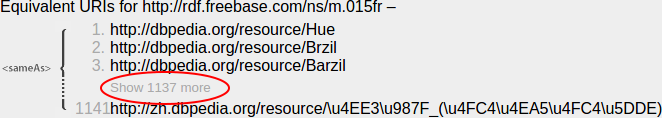
\includegraphics[width=\columnwidth]{img/sameasorg.png}
 	\caption{Several URIs with the property \qname{owl:sameAs} from the web site sameAs.org.}
  	\label{fig:sameasorg}
\end{figure}

Our work is not an alternative to the sameAs web site, but brings possibilities, like, was noticed that the sameAs.org does not provide a way to rate the link, but with this rating, is possible to improve the quality of the data, and bring some facility to the user.

\section{Detection of Erroneous Links in Large-Scale RDF Datasets}
Our work has the aim of detecting erroneous links in large-scale link repositories improving the consistency. The state-of-the-art include the following related works:

%Since 1980, the Oracle database has implemented an extension of SQL by the instructions CONNECT BY and START WITH, which allows the computation of a transitive closure as part of a query.
%The standard SQL 3 from 1999 uses a generic constructor with the instruction WITH RECURSIVE, allowing transitive closures being computed inside the query processor.
%In 2011, transitive closures were implemented by the IBM DB2, Microsoft SQL Server and PostgreSQL.

\begin{itemize}
	\item Albertoni et al.~\cite{Albertoni:2013:ALQ:2457317.2457327} focus on the quality dimension of completeness using scoring functions and also introduce a notion of linkset quality, considering only \texttt{owl:sameAs}. The work proposes three quality indicators to assess completeness. The extension of this work~\cite{albertoni2015linkset} focuses on \texttt{skos:exactMatch} linksets and a multilingual gain. 
	%The difference here is that the work does not investigate a \textit{scoring function} for a large linkset with many types of links, such as LinkLion~\cite{nentwig2014linklion}.
	
	%\item The approach~\cite{Albertoni:2013:ALQ:2457317.2457327} brings the concept of Linkset Type Completeness, the ability of detecting incompleteness of strongly depends on correctness of the type equivalence relation, but only for reflexive and symmetric closures. \todo{Need just to ajust this text...}
	
	\item The LINK-QA tool~\cite{Guret2012AssessingLD} uses two network measures designed for Linked Data (i.e., open \texttt{sameAs} chains, and description richness) and three classic network measures (i.e., degree, centrality, clustering coefficient) in order to determine whether a set of links can improve the quality of linked data. 
	%The work shows which linksets are good, but does not improve the linkset, also noticed by~\cite{Albertoni:2013:ALQ:2457317.2457327}.
	
	\item DBpediaSameAs~\cite{valdestilhasdbpediasameas} is a work in which Transitive Redirects Links are redundancies at DBpedia that supposes a link to the same place, in other words, they use the \texttt{owl:sameAs} property. These links will redirect other links, to provide a transition between the links, hence the name transitive. In this case, instead of using the transitive links that point to the same final destination URI, the final URI is used directly. 
	%In a certain way, they provide the transitive closure, but not reflexive and symmetric closures.
	
	\item The work proposed in~\cite{yaghouti2015metric} is a metric-driven approach for interlinking assessment of a single dataset. It introduces the concept of \emph{link-ability}, which shows the potential of a dataset being linked from other datasets, and in general, assesses whether a dataset is good to be interlinked with another dataset using three groups of metrics.
	
	\item The approach at~\cite{casanova2014materialized} proposes strategies in order to reduce the cognitive overhead of creating materialized \texttt{owl:sameAs} linksets and to correctly maintain them using two types of components that triple stores should include, which would improve the support for materialized \texttt{owl:sameAs} linksets in the creation and maintenance stages.
	
	\item~\cite{netoassessing} evaluates the quantity of links between distributions, datasets, and ontologies categorizing and defining different types of links using probabilistic data structures.
	The results show valid links, dead links, and a number of namespaces described by distributions and datasets. The analysis was conducted using LODVader~\cite{baron2016lodvader}.
	An important point here and in works such as~\cite{scharffe2009rdf,beek2014lod,makela2014aether} is that they do not mention or use any quality dimension as defined in some important works such as~\cite{zaveri2015quality,albertoni2015linkset}; moreover, they do not consider the axioms related to the properties. The quality is given solely by the number of links between datasets.
	
	%\item BioPortal~\cite{noy2009bioportal} is a project more related to LinkLion, where the main difference is instead of store relations of any type of domain, this repository was made to store biomedical ontologies. 
	
	\item The work described in~\cite{paulheim2014identifying} covers an unsupervised approach for finding erroneous links, in which each link is represented as a feature vector in a higher dimensional vector space, and finds wrong links by means of different multi-dimensional outliers.
%In other words, our work is looking for the quality dimension of consciousness of linksets, not datasets.
	
	\item The W3C has a vocabulary to express the quality of data, including a linkset\footnote{\url{https://w3c.github.io/dwbp/vocab-dqg.html\#ExpressQualLinkset}}, that is based on the survey by Zaveri et al.~\cite{zaveri2015quality}.
	
	\item The work described in~\cite{albertoni2016linkset} discuss results of quality evaluation on linksets created using a framework called LusTRE with two quality measures, the \textit{average linkset reachability} and the \textit{average linkset importing}. 
    Similar to CEDAL, this work realizes that the research on Linked Data quality has been mainly focused on datasets, not on linksets.
	However, they focus on the \texttt{SKOS}\footnote{\url{https://www.w3.org/2004/02/skos/}} vocabulary, more precisely \texttt{skos:exactMatch} linksets, and the experiments from CEDAL were processed in large scale link repositories with more than $10^7$ triples, not only $31,298$ triples. 
	
	\item The work described in~\cite{Melo2013NotQT} provides an algorithm with the intention to mitigate the problem of constraints violations in sameAs links automatically. Our approach has some different characteristics, such as CEDAL provides a classification of errors and show that some of them cannot be dealt with automatically in an accurate way, CEDAL use graph partitions in which scales better than this existing approach. This is also shown by the evaluation of CEDAL on larger datasets (19 million vs 3 million), CEDAL preserves the provenance of the links,  CEDAL does not remove automatically constraints violations due to the fact that the output results involves semantic accuracy and thus needs human feedback. The similarities include the fact that we also focus on owl:sameAs and we reveal a significant amount of sameAs links that do not adhere to the strict semantics of the OWL standard and hence do not reflect genuine identity.
\end{itemize}
%
Common points among these existing works are the improvement and maintenance of link repositories. Aspects include the use of scoring functions, transitive and redirect links, metrics for interlinking datasets, probabilistic data structures, vector space models, and the creation of standards. Our approach provides a high-performance way to dealing with heterogeneous knowledge bases showing the provenance and detecting inconsistent links in large-scale link repositories. 
Although our work bears some resemblance to existing work on detecting erroneous link candidates in large link repositories, none of the above has considered evaluating the consistency of equivalence relations using a data quality measure. % showing the provenance of these links, allowing a significant improvement in these link repositories. 

The novelty of CEDAL with respect to the state-of-the-art can be enumerated in five points. Our approach (1) uses graph partitions and hence scales better than existing approaches using closures, (2) can be applied to larger linksets, with more than 19 million triples, (3) preserves the provenance of the links, (4) shows that some of the error classifications cannot be dealt with automatically in an accurate way and (5) does not remove automatically constraints violations due to the fact that the output results involves semantic accuracy and thus needs human feedback.

\section{Querying Large Heterogeneous RDF Datasets}
In this section, we provide a brief overview of the state-of-the-art pertaining to querying a huge amount of heterogeneous LOD datasets, in which we start with approaches for federated query processing.
\paragraph*{\textbf{Query federation over multiple SPARQL endpoints:}}

DARQ \cite{darq2008}, ADERIS \cite{aderis2011}, FedX \cite{fedx2011}, Lusail \cite{abdelaziz2017lusail}, SPLENDID \cite{splendid2011}, CostFed \cite{saleem2018costfed}, ANAPSID \cite{anapsid2011}, SemaGrow \cite{semagrow2015}, Odyssey \cite{odyssey2017}, and MULDER \cite{endris2018querying} are examples of state-of-the-art SPARQL endpoint federation engines. These approaches can be further divided into 3 categories namely \emph{index-only}, \emph{index-free}, and hybrid (index+\texttt{ASK}) approaches \cite{saleem2015fine}. 

DARQ and ADERIS are examples of the index-only SPARQL query federation approaches over multiple SPARQL endpoints. DARQ implements a cardinality-based query planner with bind join implementation in nested loops. ADERIS is an adaptive query engine that implements a cost-based query planner. It also makes use of the index-based nested loop join. 

FedX and Lusail are examples of the index-free query federation approaches over multiple SPARQL endpoints. 
FedX only makes use of \texttt{ASK} queries for source selection. It implements a heuristic-based query planner. Comparing to DARQ, the number of endpoints requests is greatly reduced by using bind joins in a block nested loop fashion \cite{fedx2011}. A query rewriting algorithm is used to
push computation to the local endpoints by relying on information about the underlying RDF datasets. It implements a selectivity-aware query execution plan generation. 

SPLENDID, CostFed, ANAPSID, SemaGrow, and Odyssey are examples of the hybrid (index+\texttt{ASK}) SPARQL query federation approaches over multiple SPARQL endpoints. SPLENDID performs cost-based optimization using VOID statistics from datasets. It makes use of bind and hash joins \cite{saleem2015fine}. %A dynamic programming strategy~\cite{key-42} is used for join ordering. 
CostFed also implements a cost-based query planner. The source selection is closely related to HiBISCuS \cite{hibiscus2014}. Both bind and symmetric hash joins are used for data integration. ANAPSID \cite{anapsid2011} is an adaptive query federation engine that adapts its query execution at runtime according to the data availability and condition of the SPARQL endpoints.  ANAPSID implements adaptive group and adaptive dependent joins \cite{saleem2015fine}. SemaGrow adapts source selection approach from SPLENDID. It performs a cost-based query planning based on VOID statistics about datasets. SemaGrow implements bind, hash, and merge joins. Odyssey is also a cost-based federation engine. MULDER describes data sources in terms of RDF molecule templates and utilize these template for source selection, and query decomposition and optimization.

DAW \cite{daw2013} 
and Fedra \cite{fedra2015} are examples of duplicate-aware query federation approaches over multiple SPARQL endpoints. 

SaGe\cite{DBLP:journals/corr/abs-1806-00227} is a stateless preemptable SPARQL query engine for public endpoints. The system makes use of preemptable query plans and time-sharing scheduling, SaGe tackles the problem of RDF data availability for complex queries in public endpoints. Consequently, SaGe provides a convenient alternative to the current practice of copying RDF data dumps.

\paragraph*{\textbf{Link Traversal based SPARQL federation:}} LDQPS~\cite{ldqp2010}, SIHJoin~\cite{sihjoin2011}, WoDQA~\cite{wodqa2012}, and SQUIN~\cite{hartig2013squin} are examples of traversal-based federated SPARQL query processing approaches.  
Both LQPS and SIHJoin make use of the index and  online discovery via link-traversal to identify the relevant sources pertaining to the given SPARQL query. They implement symmetric hash join. WoDQA performs hybrid (index+\texttt{ASK}) source selection approach. It implements nested loop and bind joins. SQUIN discovers the potentially relevant data during the query execution and thus produce incremental query results. SQUIN uses a heuristic for query execution plan generation, adapted from \cite{zk2011}. As a physical implementation of the logical plans, SQUIN uses a synchronized pipeline of iterators such that the i-th operator is responsible for the i-th triple pattern of the given SPARQL query. More recent studies \cite{hartig2016walking} investigated 14 different approaches to rank traversal steps and achieve a variety of traversal strategies. 
A more exhaustive survey of the traversal-based SPARQ query federation is provided in \cite{hartig2009executing}. 

Beside the above query federation strategies, low-cost triple pattern fragments (TPF) interfaces \cite{verborgh2016triple} can also be used to execute federated SPARQL queries. Comunica~\cite{taelman2018comunica} is a highly modular meta engine for federated SPARQL query evaluation over support heterogeneous interfaces types, including self-descriptive Linked Data interfaces such as TPF. The system also enables querying over heterogeneous sources, such as SPARQL endpoints and data dumps in RDF serializations. The main drawback here is that the user should know in advance the dataset where the query will be executed.

One of the targets and motivation to build WimuQ was to discover which dataset the SPARQL query can be executed, unfortunately, with exception of SQUIN~\cite{hartig2013squin}, none of the related works provides this feature. Despite the fact that some of them incorporate Nquad support that allows the possibility to know the graph of the triple. The provenance system of WimuQ also includes dump files and endpoints with a rank provided by WIMU~\cite{valdestilhas2018my}.